\documentclass[12pt, titlepage]{article}

\usepackage{booktabs}
\usepackage{tabularx}
\usepackage{hyperref}
\hypersetup{
    colorlinks,
    citecolor=black,
    filecolor=black,
    linkcolor=red,
    urlcolor=blue
}
\usepackage[round]{natbib}
\usepackage{enumitem}
\usepackage{tikz}
\usetikzlibrary{automata,positioning,arrows}

\title{SE 4G06: Software Requirements Specification\\Team \#12 - CodeChamp}

\author{
  Kanugalawattage, Anton
  \and
  Subedi, Dipendra
  \and
  Rizkalla, Youssef
  \and
  Leung, Tamas
  \and
  Zhao, Zhiming
}


\date{\today}

\input{../Common}
\input{../Comments}

\begin{document}

\maketitle

\pagenumbering{roman}
\tableofcontents
\listoftables
\listoffigures

\begin{table}[bp]
\caption{\bf Revision History}
\begin{tabularx}{\textwidth}{p{3cm}p{2cm}X}
\toprule {\bf Date} & {\bf Version} & {\bf Notes}\\
\midrule
Sept. 27, 2022 & 0.1 & Initial Version\\
\bottomrule
\end{tabularx}
\end{table}


\newpage

\pagenumbering{arabic}

% This document describes the requirements for ....  The template for the Software
% Requirements Specification (SRS) is a subset of the Volere
% template~\citep{RobertsonAndRobertson2012}.  If you make further modifications
% to the template, you should explicity state what modifications were made.



\section{Project Drivers}

\subsection{The Purpose of the Project}

Practicing coding the traditional way can be daunting. The current most popular method to learn is to use a problem database site like \href{http://www.leetcode.com}{LeetCode}. This method of learning can often feel tiring and endless. There are over 2000 problems on the website which can be intimidating to many new coders. CodeChamp will introduce a collaborative and fun way to interact with your friends while improving your algorithmic skills.

\subsection{The Stakeholders}

\subsubsection{The Client}
\begin{itemize}
    \item Dr. Spencer Smith
    \item TAs of SE 4G06
\end{itemize}

\subsubsection{The Customers}
\begin{itemize}
    \item Learners who wants to practice and improve on their data structures \& algorithmic skills.
    \item Existing users of popular coding practice sites like Leetcode and DMOJ.
    \item Groups looking to compete and practice their coding skills.
\end{itemize}

\subsubsection{Other Stakeholders}
\begin{itemize}
    \item Developers on the project
\end{itemize}

\subsection{Mandated Constraints}

\subsubsection{Solution Constraints}
\begin{itemize}
    \item System shall be accessible through the internet to any device with a browser.
\end{itemize}

\subsubsection{Budget Constraints}
\begin{itemize}
    \item For the scope of the project, deployment and hosting shall cost \$0.
\end{itemize}

\subsection{Naming Conventions and Terminology}
\begin{itemize}
    \item 
\end{itemize}

\subsection{Relevant Facts and Assumptions}
\begin{itemize}
    \item User's have and will maintain a steady internet connection throughout the game.
    \item User's will have input devices to type out their solutions to the problems presented. 
    \item User is able to navigate a computer or a smart device.
\end{itemize}

\section{Functional Requirements}

\subsection{The Scope of the Work and the Product}

\subsubsection{The Context of the Work}
\begin{itemize} 
    \item This application will allow 2-20 users in a lobby to compete against each other across multiple browsers.
\end{itemize}

\subsubsection{Work Partitioning}
\begin{itemize} 
    \item Server will maintain all match data
    \item Server will compile user's submissions and evaluate the correctness of the submission. 
    \item User clients will request match data and match state from server
    \item User clients will communicate with server to update match state
\end{itemize}

\subsubsection{Individual Product Use Cases}
\begin{itemize} 
    \item{User creates an account}
    \item{User logins into application}
    \item{User creates a lobby}
    \item{User creates invite code to invite friends}
    \item{User joins lobby with an invite code}
    \item{User finds lobby to join}
    \item{User writes code in editor}
    \item{User submits code for compilation}
    \item{User returns to main menu after winning/losing}
    \item{User views previous match history}
\end{itemize}

\subsection{Functional Requirements}
\begin{enumerate}[label=FR.\arabic*]
    \item The system shall allow users to sign up using a username, email and password.
    \item The system shall allow users to log in using a username and password.
    \item The system shall display an error if the user fails to log in.
    \item The system shall allow users to create a lobby link.
    \item The system shall allow users to join a lobby using a link.
    \item The system shall match-make users into a match.
    \item The system shall start a match when 20 players are match-made.
    \item The system shall have 3 rounds per match.
    \item The system shall display one coding problem per round.
    \item The system shall allow users to submit code through the web interface.
    \item The system shall compile the user's code.
    \item The system shall detect malicious code.
    \item The system shall prevent malicious code from compiling.
    \item The system shall display the result of the code's compilation and report any errors to the user.
    \item The system shall run the user's code against the test cases for a problem.
    \item The system shall track the code's running time in seconds and its memory usage in megabytes.
    \item The system shall time-out any code that exceeds the time or memory limit for a coding problem.
    \item The system shall display the result of running the user's code against the test cases to the user.
    \item The system shall qualify the first 10 users in the first round to solve the coding problem into the second round and shall disqualify the remainder.
    \item The system shall qualify the first 5 users in the second round to solve the coding problem into the third round and shall disqualify the remainder.
    \item The system shall declare the first user to solve the coding problem in the final round as the winner and shall disqualify the remainder.
    \item The system shall allow users to view a history of their previous matches.
    \item The system shall display the user's win percentage.
    \item The system shall display the rounds in which the users qualified or disqualified for a match's history.
    \item The system shall display the coding problem for each round in a match's history.
    \item The system shall track and display the top 100 users with the largest number of wins.
    \item The system shall allow developers to create, modify and delete coding problems.
    \item The system shall allow developers to create, modify and delete test cases for a coding problem.
    \item The system shall allow developers to define a time in seconds and a memory limit in megabytes for each coding problem.
\end{enumerate}

\subsection{User Lobby State Flow}
%% Machine generated by https://finsm.io
%% 2022-9-27-20:08:038
\begin{center}
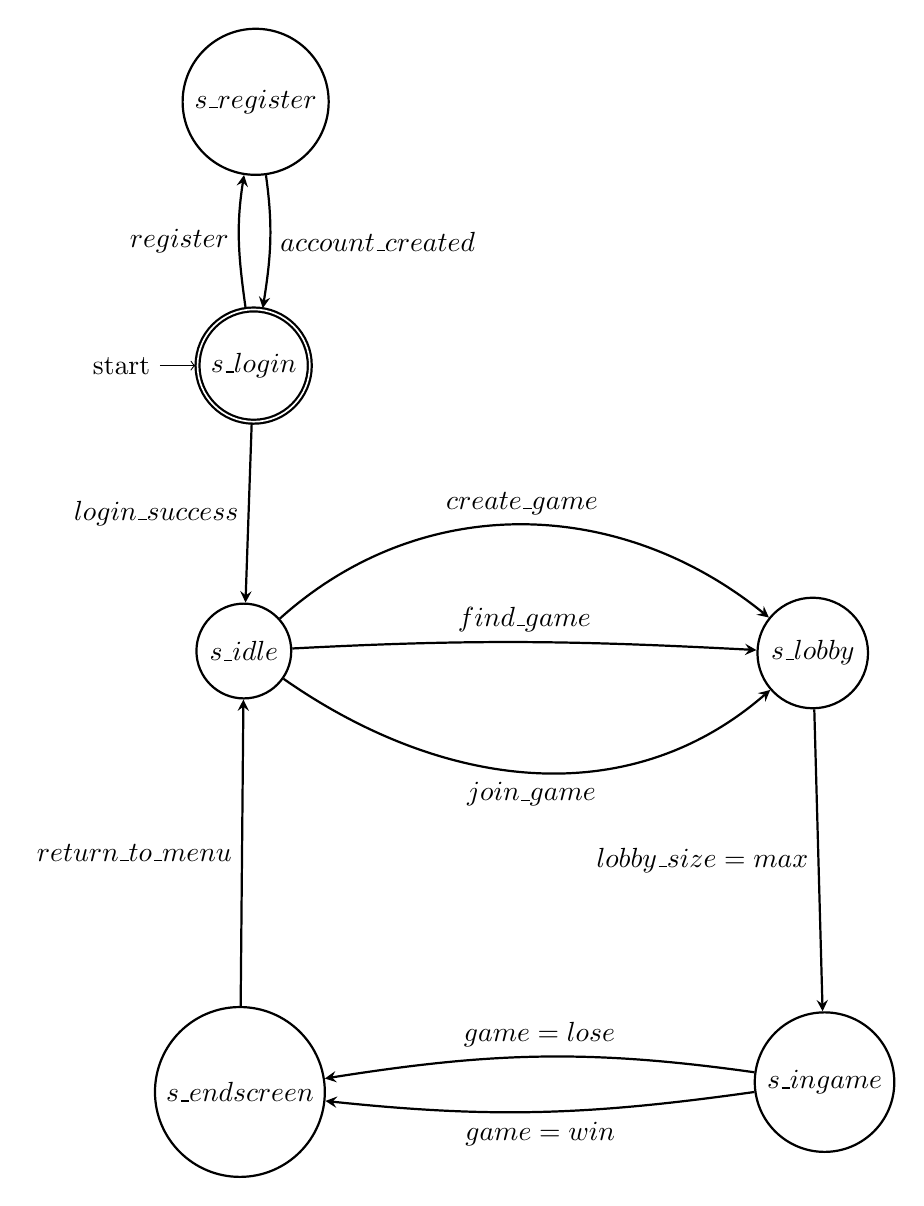
\begin{tikzpicture}[]
    \node[initial,thick,accepting,state] at (-3.9,4.175) (2a413fb1) {$s\_login$};
    \node[thick,state] at (-3.875,7.525) (291d825b) {$s\_register$};
    \node[thick,state] at (-4.025,0.55) (e39a07c9) {$s\_idle$};
    \node[thick,state] at (3.2,0.525) (981cc1fb) {$s\_lobby$};
    \node[thick,state] at (3.35,-4.925) (d4f7f4ce) {$s\_ingame$};
    \node[thick,state] at (-4.075,-5.05) (21148f7e) {$s\_endscreen$};
    \path[->, thick, >=stealth]
    (2a413fb1) edge [left,in = -99, out = 98] node {$register$} (291d825b)
    (2a413fb1) edge [left] node {$login\_success$} (e39a07c9)
    (291d825b) edge [right,in = 81, out = -82] node {$account\_created$} (2a413fb1)
    (e39a07c9) edge [above,in = 141, out = 42] node {$create\_game$} (981cc1fb)
    (e39a07c9) edge [above,in = 177, out = 3] node {$find\_game$} (981cc1fb)
    (e39a07c9) edge [below,in = -139, out = -35] node {$join\_game$} (981cc1fb)
    (981cc1fb) edge [left] node {$lobby\_size=max$} (d4f7f4ce)
    (d4f7f4ce) edge [above,in = 9, out = 172] node {$game=lose$} (21148f7e)
    (d4f7f4ce) edge [below,in = -6, out = -172] node {$game=win$} (21148f7e)
    (21148f7e) edge [left] node {$return\_to\_menu$} (e39a07c9)
    ;
\end{tikzpicture}
\end{center}

\section{Non-functional Requirements}

\subsection{Look and Feel Requirements}
\begin{enumerate}[label=NFR.\arabic*]
    \item The interface of the system shall be easy to read and the elements are not clumped together.
    \item The elements on the interface shall be organized and placed in a logical way.
\end{enumerate}

\subsection{Usability and Humanity Requirements}
\begin{enumerate}[label=NFR.\arabic*, resume]
    \item People with basic computer understanding shall be able to navigate the system.
    \item The system shall be simple to understand and user should spend less than 5 minutes to understand what each part of the system does. 
    \item The system should be easily accessible so that the user can navigate around the system without the use of mouse.
\end{enumerate}
\subsection{Performance Requirements}
\begin{enumerate}[label=NFR.\arabic*, resume]
    \item The system shall respond to a user's action within 2 seconds.
    \item The system shall process and give results base on user's inputs within 10 seconds.
    \item The system shall be operating 24 hours a day, 7 days a week.
\end{enumerate}
\subsection{Operational and Environmental Requirements}
\begin{enumerate}[label=NFR.\arabic*, resume]
    \item The system should run on major browsers and devices that support these browsers.
\end{enumerate}
\subsection{Maintainability and Support Requirements}
\begin{enumerate}[label=NFR.\arabic*, resume]
    \item The system shall provide the ability for developers to add questions and test cases when needed.
\end{enumerate}
\subsection{Security Requirements}
\begin{enumerate}[label=NFR.\arabic*, resume]
    \item The system shall require users to register their own accounts in order to use the system.
    \item The system shall deny the user access if the user fails to login.
\end{enumerate}
\subsection{Cultural Requirements}
\begin{enumerate}[label=NFR.\arabic*, resume]
    \item The system shall not have anything that is or suggests cultural inappropriate content. 
\end{enumerate}
\subsection{Legal Requirements}
\begin{enumerate}[label=NFR.\arabic*, resume]
    \item The system shall be protected by GNU General Public License (GPL). 
\end{enumerate}
\subsection{Health and Safety Requirements}
\begin{enumerate}[label=NFR.\arabic*, resume]
    \item The system shall not have any flashing lights that can put the user under the risk of epilepsy or seizure.
\end{enumerate}
% This section is not in the original Volere template, but health and safety are
% issues that should be considered for every engineering project.

\section{Project Issues}

\subsection{Open Issues} 
\begin{itemize} 
    \item Judging and evaluation of a user submission
    \item Safety, managing malicious code submissions
\end{itemize}

\subsection{Off-the-Shelf Solutions}
N/A

\subsection{New Problems}
N/A

\subsection{Tasks}
\begin{itemize} 
    \item Back-end architecture design
    \item Front-end UI design
    \item Communication schema design between front-end and back-end
    \item Database schema design
    \item Unit tests for front-end and back-end
    \item End to End integration tests
\end{itemize}

\subsection{Migration to the New Product}
N/A

\subsection{Risks}
\begin{itemize}
    \item Multiple concurrent communications between front-end and back-end
    \item Back-end server may not be able to handle multiple concurrent of compilation
    \item Distributed Denial-of-Service attacks
    \item Malicious code injections
\end{itemize}

\subsection{Costs}
\begin{itemize}
    \item Back-end hosting server costs
    \item Front-end hosting server costs
    \item Database hosting costs
\end{itemize}

\subsection{User Documentation and Training}
N/A

\subsection{Waiting Room}
N/A

\subsection{Ideas for Solutions}
For concurrent communications and concurrent code compilations, vertical scaling for hardware is an easy fast method to remove the limitations of concurrency. However this leads to future higher costs. Load balancing can be used to allow for horizontal scaling of system.

For costs, many options exists for free/hobby tier project hosting, allowing for cost savings.

\bibliographystyle{plainnat}

\bibliography{SRS}

\newpage

\section{Appendix}

This section has been added to the Volere template.  This is where you can place
additional information.

\subsection{Symbolic Parameters}

The definition of the requirements will likely call for SYMBOLIC\_CONSTANTS.
Their values are defined in this section for easy maintenance.


\end{document}
